\documentclass{standalone}
\usepackage{tikz}
\usetikzlibrary{patterns, positioning}


\begin{document}
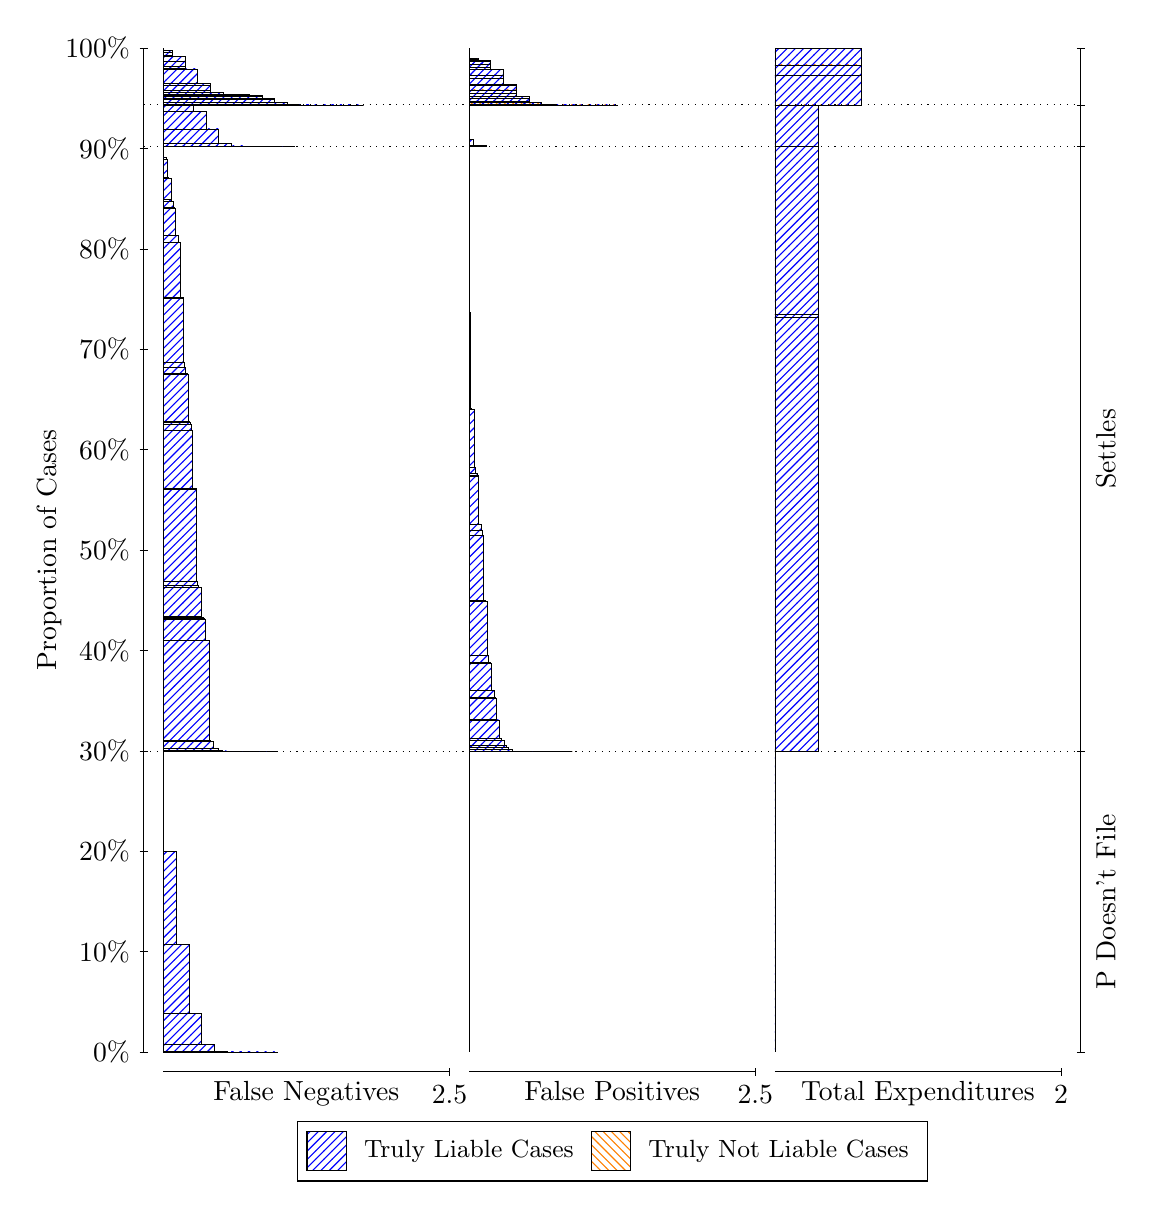
\begin{tikzpicture}
\draw[black, very thin] (1.5,1.75) -- (1.5,14.5);
\node[rotate=90, text=black, anchor=center] at (0.3, 8.125) {Proportion of Cases};
\draw[black, very thin] (1.45,1.75) -- (1.55,1.75);
\node[text=black, anchor=east] at (1.45, 1.75) {0\%};
\draw[black, very thin] (1.45,3.025) -- (1.55,3.025);
\node[text=black, anchor=east] at (1.45, 3.025) {10\%};
\draw[black, very thin] (1.45,4.3) -- (1.55,4.3);
\node[text=black, anchor=east] at (1.45, 4.3) {20\%};
\draw[black, very thin] (1.45,5.575) -- (1.55,5.575);
\node[text=black, anchor=east] at (1.45, 5.575) {30\%};
\draw[black, very thin] (1.45,6.85) -- (1.55,6.85);
\node[text=black, anchor=east] at (1.45, 6.85) {40\%};
\draw[black, very thin] (1.45,8.125) -- (1.55,8.125);
\node[text=black, anchor=east] at (1.45, 8.125) {50\%};
\draw[black, very thin] (1.45,9.4) -- (1.55,9.4);
\node[text=black, anchor=east] at (1.45, 9.4) {60\%};
\draw[black, very thin] (1.45,10.675) -- (1.55,10.675);
\node[text=black, anchor=east] at (1.45, 10.675) {70\%};
\draw[black, very thin] (1.45,11.95) -- (1.55,11.95);
\node[text=black, anchor=east] at (1.45, 11.95) {80\%};
\draw[black, very thin] (1.45,13.225) -- (1.55,13.225);
\node[text=black, anchor=east] at (1.45, 13.225) {90\%};
\draw[black, very thin] (1.45,14.5) -- (1.55,14.5);
\node[text=black, anchor=east] at (1.45, 14.5) {100\%};

\draw[black, very thin] (13.4,1.75) -- (13.4,14.5);
\draw[black, very thin] (13.35,1.75) -- (13.45,1.75);
\node[anchor=west] at (13.35, 1.75) {};
\draw[black, very thin] (13.35,5.563) -- (13.45,5.563);
\node[anchor=west] at (13.35, 5.563) {};
\draw[black, very thin] (13.35,13.254) -- (13.45,13.254);
\node[anchor=west] at (13.35, 13.254) {};
\draw[black, very thin] (13.35,13.779) -- (13.45,13.779);
\node[anchor=west] at (13.35, 13.779) {};
\draw[black, very thin] (13.35,14.5) -- (13.45,14.5);
\node[anchor=west] at (13.35, 14.5) {};

\draw[black, very thin, pattern color=blue, pattern=north east lines] (1.75,1.75) rectangle (3.2033,1.75);
\draw[black, very thin, pattern color=blue, pattern=north east lines] (1.75,1.75) rectangle (3.0419,1.75);
\draw[black, very thin, pattern color=blue, pattern=north east lines] (1.75,1.75) rectangle (2.8804,1.75);
\draw[black, very thin, pattern color=blue, pattern=north east lines] (1.75,1.75) rectangle (2.7189,1.7503);
\draw[black, very thin, pattern color=blue, pattern=north east lines] (1.75,1.7503) rectangle (2.5574,1.7582);
\draw[black, very thin, pattern color=blue, pattern=north east lines] (1.75,1.7582) rectangle (2.3959,1.8434);
\draw[black, very thin, pattern color=blue, pattern=north east lines] (1.75,1.8434) rectangle (2.2344,2.2366);
\draw[black, very thin, pattern color=blue, pattern=north east lines] (1.75,2.2366) rectangle (2.073,3.1157);
\draw[black, very thin, pattern color=blue, pattern=north east lines] (1.75,3.1157) rectangle (1.9115,4.2995);
\draw[black, very thin, pattern color=orange, pattern=north west lines] (1.75,4.2995) rectangle (1.75,4.2995);
\draw[black, very thin, pattern color=blue, pattern=north east lines] (1.75,4.2995) rectangle (1.75,5.563);
\draw[black, very thin, pattern color=blue, pattern=north east lines] (1.75,5.563) rectangle (3.2033,5.563);
\draw[black, very thin, pattern color=blue, pattern=north east lines] (1.75,5.563) rectangle (3.1307,5.563);
\draw[black, very thin, pattern color=blue, pattern=north east lines] (1.75,5.563) rectangle (3.058,5.563);
\draw[black, very thin, pattern color=blue, pattern=north east lines] (1.75,5.563) rectangle (3.0419,5.563);
\draw[black, very thin, pattern color=blue, pattern=north east lines] (1.75,5.563) rectangle (2.9853,5.563);
\draw[black, very thin, pattern color=blue, pattern=north east lines] (1.75,5.563) rectangle (2.9692,5.563);
\draw[black, very thin, pattern color=blue, pattern=north east lines] (1.75,5.563) rectangle (2.9127,5.563);
\draw[black, very thin, pattern color=blue, pattern=north east lines] (1.75,5.563) rectangle (2.8965,5.563);
\draw[black, very thin, pattern color=blue, pattern=north east lines] (1.75,5.563) rectangle (2.8804,5.563);
\draw[black, very thin, pattern color=blue, pattern=north east lines] (1.75,5.563) rectangle (2.84,5.563);
\draw[black, very thin, pattern color=blue, pattern=north east lines] (1.75,5.563) rectangle (2.8239,5.563);
\draw[black, very thin, pattern color=blue, pattern=north east lines] (1.75,5.563) rectangle (2.8077,5.563);
\draw[black, very thin, pattern color=blue, pattern=north east lines] (1.75,5.563) rectangle (2.7673,5.563);
\draw[black, very thin, pattern color=blue, pattern=north east lines] (1.75,5.563) rectangle (2.7512,5.563);
\draw[black, very thin, pattern color=blue, pattern=north east lines] (1.75,5.563) rectangle (2.735,5.563);
\draw[black, very thin, pattern color=blue, pattern=north east lines] (1.75,5.563) rectangle (2.7189,5.563);
\draw[black, very thin, pattern color=blue, pattern=north east lines] (1.75,5.563) rectangle (2.6947,5.563);
\draw[black, very thin, pattern color=blue, pattern=north east lines] (1.75,5.563) rectangle (2.6785,5.563);
\draw[black, very thin, pattern color=blue, pattern=north east lines] (1.75,5.563) rectangle (2.6624,5.563);
\draw[black, very thin, pattern color=blue, pattern=north east lines] (1.75,5.563) rectangle (2.6462,5.563);
\draw[black, very thin, pattern color=blue, pattern=north east lines] (1.75,5.563) rectangle (2.622,5.563);
\draw[black, very thin, pattern color=blue, pattern=north east lines] (1.75,5.563) rectangle (2.6059,5.5636);
\draw[black, very thin, pattern color=blue, pattern=north east lines] (1.75,5.5636) rectangle (2.5897,5.5636);
\draw[black, very thin, pattern color=blue, pattern=north east lines] (1.75,5.5636) rectangle (2.5736,5.5636);
\draw[black, very thin, pattern color=blue, pattern=north east lines] (1.75,5.5636) rectangle (2.5574,5.5638);
\draw[black, very thin, pattern color=blue, pattern=north east lines] (1.75,5.5638) rectangle (2.5493,5.5752);
\draw[black, very thin, pattern color=blue, pattern=north east lines] (1.75,5.5752) rectangle (2.5332,5.5752);
\draw[black, very thin, pattern color=blue, pattern=north east lines] (1.75,5.5752) rectangle (2.517,5.5752);
\draw[black, very thin, pattern color=blue, pattern=north east lines] (1.75,5.5752) rectangle (2.5009,5.5757);
\draw[black, very thin, pattern color=blue, pattern=north east lines] (1.75,5.5757) rectangle (2.4847,5.576);
\draw[black, very thin, pattern color=blue, pattern=north east lines] (1.75,5.576) rectangle (2.4605,5.576);
\draw[black, very thin, pattern color=blue, pattern=north east lines] (1.75,5.576) rectangle (2.4444,5.6026);
\draw[black, very thin, pattern color=blue, pattern=north east lines] (1.75,5.6026) rectangle (2.4282,5.6033);
\draw[black, very thin, pattern color=blue, pattern=north east lines] (1.75,5.6033) rectangle (2.4121,5.6038);
\draw[black, very thin, pattern color=blue, pattern=north east lines] (1.75,5.6038) rectangle (2.3959,5.6069);
\draw[black, very thin, pattern color=blue, pattern=north east lines] (1.75,5.6069) rectangle (2.3879,5.6976);
\draw[black, very thin, pattern color=blue, pattern=north east lines] (1.75,5.6976) rectangle (2.3717,5.6977);
\draw[black, very thin, pattern color=blue, pattern=north east lines] (1.75,5.6977) rectangle (2.3556,5.6985);
\draw[black, very thin, pattern color=blue, pattern=north east lines] (1.75,5.6985) rectangle (2.3394,5.7093);
\draw[black, very thin, pattern color=blue, pattern=north east lines] (1.75,5.7093) rectangle (2.3313,6.9724);
\draw[black, very thin, pattern color=blue, pattern=north east lines] (1.75,6.9724) rectangle (2.3233,6.9762);
\draw[black, very thin, pattern color=blue, pattern=north east lines] (1.75,6.9762) rectangle (2.299,6.9763);
\draw[black, very thin, pattern color=blue, pattern=north east lines] (1.75,6.9763) rectangle (2.2829,7.2447);
\draw[black, very thin, pattern color=blue, pattern=north east lines] (1.75,7.2447) rectangle (2.2667,7.2605);
\draw[black, very thin, pattern color=blue, pattern=north east lines] (1.75,7.2605) rectangle (2.2506,7.2683);
\draw[black, very thin, pattern color=blue, pattern=north east lines] (1.75,7.2683) rectangle (2.2344,7.2832);
\draw[black, very thin, pattern color=blue, pattern=north east lines] (1.75,7.2832) rectangle (2.2264,7.6522);
\draw[black, very thin, pattern color=blue, pattern=north east lines] (1.75,7.6522) rectangle (2.2102,7.6538);
\draw[black, very thin, pattern color=blue, pattern=north east lines] (1.75,7.6538) rectangle (2.1941,7.6711);
\draw[black, very thin, pattern color=blue, pattern=north east lines] (1.75,7.6711) rectangle (2.1779,7.723);
\draw[black, very thin, pattern color=blue, pattern=north east lines] (1.75,7.723) rectangle (2.1699,8.8989);
\draw[black, very thin, pattern color=blue, pattern=north east lines] (1.75,8.8989) rectangle (2.1618,8.9082);
\draw[black, very thin, pattern color=blue, pattern=north east lines] (1.75,8.9082) rectangle (2.1376,8.91);
\draw[black, very thin, pattern color=blue, pattern=north east lines] (1.75,8.91) rectangle (2.1214,9.6471);
\draw[black, very thin, pattern color=blue, pattern=north east lines] (1.75,9.6471) rectangle (2.1053,9.7219);
\draw[black, very thin, pattern color=blue, pattern=north east lines] (1.75,9.7219) rectangle (2.0891,9.7416);
\draw[black, very thin, pattern color=blue, pattern=north east lines] (1.75,9.7416) rectangle (2.073,9.7546);
\draw[black, very thin, pattern color=blue, pattern=north east lines] (1.75,9.7546) rectangle (2.0649,10.36);
\draw[black, very thin, pattern color=blue, pattern=north east lines] (1.75,10.36) rectangle (2.0487,10.367);
\draw[black, very thin, pattern color=blue, pattern=north east lines] (1.75,10.367) rectangle (2.0326,10.446);
\draw[black, very thin, pattern color=blue, pattern=north east lines] (1.75,10.446) rectangle (2.0164,10.506);
\draw[black, very thin, pattern color=blue, pattern=north east lines] (1.75,10.506) rectangle (2.0084,11.326);
\draw[black, very thin, pattern color=blue, pattern=north east lines] (1.75,11.326) rectangle (2.0003,11.33);
\draw[black, very thin, pattern color=blue, pattern=north east lines] (1.75,11.33) rectangle (1.9761,11.338);
\draw[black, very thin, pattern color=blue, pattern=north east lines] (1.75,11.338) rectangle (1.9599,12.031);
\draw[black, very thin, pattern color=blue, pattern=north east lines] (1.75,12.031) rectangle (1.9438,12.116);
\draw[black, very thin, pattern color=blue, pattern=north east lines] (1.75,12.116) rectangle (1.9276,12.124);
\draw[black, very thin, pattern color=blue, pattern=north east lines] (1.75,12.124) rectangle (1.9115,12.126);
\draw[black, very thin, pattern color=blue, pattern=north east lines] (1.75,12.126) rectangle (1.9034,12.47);
\draw[black, very thin, pattern color=blue, pattern=north east lines] (1.75,12.47) rectangle (1.8873,12.477);
\draw[black, very thin, pattern color=blue, pattern=north east lines] (1.75,12.477) rectangle (1.8711,12.56);
\draw[black, very thin, pattern color=blue, pattern=north east lines] (1.75,12.56) rectangle (1.855,12.577);
\draw[black, very thin, pattern color=blue, pattern=north east lines] (1.75,12.577) rectangle (1.8469,12.848);
\draw[black, very thin, pattern color=blue, pattern=north east lines] (1.75,12.848) rectangle (1.8388,12.849);
\draw[black, very thin, pattern color=blue, pattern=north east lines] (1.75,12.849) rectangle (1.8146,12.856);
\draw[black, very thin, pattern color=blue, pattern=north east lines] (1.75,12.856) rectangle (1.7984,13.088);
\draw[black, very thin, pattern color=blue, pattern=north east lines] (1.75,13.088) rectangle (1.7823,13.111);
\draw[black, very thin, pattern color=blue, pattern=north east lines] (1.75,13.111) rectangle (1.7661,13.111);
\draw[black, very thin, pattern color=orange, pattern=north west lines] (1.75,13.111) rectangle (1.75,13.111);
\draw[black, very thin, pattern color=blue, pattern=north east lines] (1.75,13.111) rectangle (1.75,13.254);
\draw[black, very thin, pattern color=blue, pattern=north east lines] (1.75,13.254) rectangle (3.4213,13.254);
\draw[black, very thin, pattern color=blue, pattern=north east lines] (1.75,13.254) rectangle (3.2599,13.254);
\draw[black, very thin, pattern color=blue, pattern=north east lines] (1.75,13.254) rectangle (3.0984,13.254);
\draw[black, very thin, pattern color=blue, pattern=north east lines] (1.75,13.254) rectangle (2.9369,13.254);
\draw[black, very thin, pattern color=blue, pattern=north east lines] (1.75,13.254) rectangle (2.7754,13.256);
\draw[black, very thin, pattern color=blue, pattern=north east lines] (1.75,13.256) rectangle (2.6139,13.292);
\draw[black, very thin, pattern color=blue, pattern=north east lines] (1.75,13.292) rectangle (2.4524,13.473);
\draw[black, very thin, pattern color=blue, pattern=north east lines] (1.75,13.473) rectangle (2.291,13.692);
\draw[black, very thin, pattern color=blue, pattern=north east lines] (1.75,13.692) rectangle (2.1295,13.768);
\draw[black, very thin, pattern color=blue, pattern=north east lines] (1.75,13.768) rectangle (1.968,13.779);
\draw[black, very thin, pattern color=orange, pattern=north west lines] (1.75,13.779) rectangle (1.75,13.779);
\draw[black, very thin, pattern color=blue, pattern=north east lines] (1.75,13.779) rectangle (4.2933,13.779);
\draw[black, very thin, pattern color=blue, pattern=north east lines] (1.75,13.779) rectangle (4.1319,13.779);
\draw[black, very thin, pattern color=blue, pattern=north east lines] (1.75,13.779) rectangle (3.9704,13.779);
\draw[black, very thin, pattern color=blue, pattern=north east lines] (1.75,13.779) rectangle (3.8089,13.779);
\draw[black, very thin, pattern color=blue, pattern=north east lines] (1.75,13.779) rectangle (3.8089,13.779);
\draw[black, very thin, pattern color=blue, pattern=north east lines] (1.75,13.779) rectangle (3.6474,13.779);
\draw[black, very thin, pattern color=blue, pattern=north east lines] (1.75,13.779) rectangle (3.6474,13.779);
\draw[black, very thin, pattern color=blue, pattern=north east lines] (1.75,13.779) rectangle (3.4859,13.783);
\draw[black, very thin, pattern color=blue, pattern=north east lines] (1.75,13.783) rectangle (3.4779,13.783);
\draw[black, very thin, pattern color=blue, pattern=north east lines] (1.75,13.783) rectangle (3.3244,13.789);
\draw[black, very thin, pattern color=blue, pattern=north east lines] (1.75,13.789) rectangle (3.3244,13.806);
\draw[black, very thin, pattern color=blue, pattern=north east lines] (1.75,13.806) rectangle (3.3164,13.806);
\draw[black, very thin, pattern color=blue, pattern=north east lines] (1.75,13.806) rectangle (3.163,13.813);
\draw[black, very thin, pattern color=blue, pattern=north east lines] (1.75,13.813) rectangle (3.163,13.844);
\draw[black, very thin, pattern color=blue, pattern=north east lines] (1.75,13.844) rectangle (3.163,13.857);
\draw[black, very thin, pattern color=blue, pattern=north east lines] (1.75,13.857) rectangle (3.1549,13.857);
\draw[black, very thin, pattern color=blue, pattern=north east lines] (1.75,13.857) rectangle (3.1549,13.857);
\draw[black, very thin, pattern color=blue, pattern=north east lines] (1.75,13.857) rectangle (3.0015,13.891);
\draw[black, very thin, pattern color=blue, pattern=north east lines] (1.75,13.891) rectangle (3.0015,13.897);
\draw[black, very thin, pattern color=blue, pattern=north east lines] (1.75,13.897) rectangle (2.9934,13.897);
\draw[black, very thin, pattern color=blue, pattern=north east lines] (1.75,13.897) rectangle (2.9934,13.897);
\draw[black, very thin, pattern color=blue, pattern=north east lines] (1.75,13.897) rectangle (2.84,13.907);
\draw[black, very thin, pattern color=blue, pattern=north east lines] (1.75,13.907) rectangle (2.8319,13.907);
\draw[black, very thin, pattern color=blue, pattern=north east lines] (1.75,13.907) rectangle (2.6785,13.908);
\draw[black, very thin, pattern color=blue, pattern=north east lines] (1.75,13.908) rectangle (2.6704,13.911);
\draw[black, very thin, pattern color=blue, pattern=north east lines] (1.75,13.911) rectangle (2.517,13.911);
\draw[black, very thin, pattern color=blue, pattern=north east lines] (1.75,13.911) rectangle (2.509,13.914);
\draw[black, very thin, pattern color=blue, pattern=north east lines] (1.75,13.914) rectangle (2.509,13.939);
\draw[black, very thin, pattern color=blue, pattern=north east lines] (1.75,13.939) rectangle (2.3556,13.939);
\draw[black, very thin, pattern color=blue, pattern=north east lines] (1.75,13.939) rectangle (2.3475,13.939);
\draw[black, very thin, pattern color=blue, pattern=north east lines] (1.75,13.939) rectangle (2.3475,13.961);
\draw[black, very thin, pattern color=blue, pattern=north east lines] (1.75,13.961) rectangle (2.3475,14.026);
\draw[black, very thin, pattern color=blue, pattern=north east lines] (1.75,14.026) rectangle (2.3475,14.054);
\draw[black, very thin, pattern color=blue, pattern=north east lines] (1.75,14.054) rectangle (2.1941,14.054);
\draw[black, very thin, pattern color=blue, pattern=north east lines] (1.75,14.054) rectangle (2.186,14.057);
\draw[black, very thin, pattern color=blue, pattern=north east lines] (1.75,14.057) rectangle (2.186,14.236);
\draw[black, very thin, pattern color=blue, pattern=north east lines] (1.75,14.236) rectangle (2.0245,14.249);
\draw[black, very thin, pattern color=blue, pattern=north east lines] (1.75,14.249) rectangle (2.0245,14.269);
\draw[black, very thin, pattern color=blue, pattern=north east lines] (1.75,14.269) rectangle (2.0245,14.328);
\draw[black, very thin, pattern color=blue, pattern=north east lines] (1.75,14.328) rectangle (2.0245,14.389);
\draw[black, very thin, pattern color=blue, pattern=north east lines] (1.75,14.389) rectangle (1.863,14.41);
\draw[black, very thin, pattern color=blue, pattern=north east lines] (1.75,14.41) rectangle (1.863,14.448);
\draw[black, very thin, pattern color=blue, pattern=north east lines] (1.75,14.448) rectangle (1.863,14.47);
\draw[black, very thin, pattern color=orange, pattern=north west lines] (1.75,14.47) rectangle (1.75,14.47);
\draw[black, very thin, pattern color=blue, pattern=north east lines] (1.75,14.47) rectangle (1.75,14.5);
\draw[black, very thin, pattern color=orange, pattern=north west lines] (5.6333,1.75) rectangle (5.6333,1.75);
\draw[black, very thin, pattern color=blue, pattern=north east lines] (5.6333,1.75) rectangle (5.6333,5.563);
\draw[black, very thin, pattern color=orange, pattern=north west lines] (5.6333,5.563) rectangle (6.9413,5.563);
\draw[black, very thin, pattern color=blue, pattern=north east lines] (5.6333,5.563) rectangle (6.9413,5.563);
\draw[black, very thin, pattern color=blue, pattern=north east lines] (5.6333,5.563) rectangle (6.7799,5.563);
\draw[black, very thin, pattern color=orange, pattern=north west lines] (5.6333,5.563) rectangle (6.7233,5.563);
\draw[black, very thin, pattern color=blue, pattern=north east lines] (5.6333,5.563) rectangle (6.7233,5.563);
\draw[black, very thin, pattern color=orange, pattern=north west lines] (5.6333,5.563) rectangle (6.6507,5.563);
\draw[black, very thin, pattern color=blue, pattern=north east lines] (5.6333,5.563) rectangle (6.6507,5.563);
\draw[black, very thin, pattern color=blue, pattern=north east lines] (5.6333,5.563) rectangle (6.6184,5.563);
\draw[black, very thin, pattern color=orange, pattern=north west lines] (5.6333,5.563) rectangle (6.578,5.563);
\draw[black, very thin, pattern color=blue, pattern=north east lines] (5.6333,5.563) rectangle (6.578,5.563);
\draw[black, very thin, pattern color=blue, pattern=north east lines] (5.6333,5.563) rectangle (6.5619,5.563);
\draw[black, very thin, pattern color=orange, pattern=north west lines] (5.6333,5.563) rectangle (6.5053,5.563);
\draw[black, very thin, pattern color=blue, pattern=north east lines] (5.6333,5.563) rectangle (6.5053,5.563);
\draw[black, very thin, pattern color=blue, pattern=north east lines] (5.6333,5.563) rectangle (6.4892,5.563);
\draw[black, very thin, pattern color=blue, pattern=north east lines] (5.6333,5.563) rectangle (6.4569,5.563);
\draw[black, very thin, pattern color=orange, pattern=north west lines] (5.6333,5.563) rectangle (6.4327,5.563);
\draw[black, very thin, pattern color=blue, pattern=north east lines] (5.6333,5.563) rectangle (6.4327,5.563);
\draw[black, very thin, pattern color=blue, pattern=north east lines] (5.6333,5.563) rectangle (6.4165,5.563);
\draw[black, very thin, pattern color=blue, pattern=north east lines] (5.6333,5.563) rectangle (6.4004,5.5631);
\draw[black, very thin, pattern color=orange, pattern=north west lines] (5.6333,5.5631) rectangle (6.36,5.5631);
\draw[black, very thin, pattern color=blue, pattern=north east lines] (5.6333,5.5631) rectangle (6.36,5.5631);
\draw[black, very thin, pattern color=blue, pattern=north east lines] (5.6333,5.5631) rectangle (6.3439,5.5639);
\draw[black, very thin, pattern color=blue, pattern=north east lines] (5.6333,5.5639) rectangle (6.3277,5.5639);
\draw[black, very thin, pattern color=blue, pattern=north east lines] (5.6333,5.5639) rectangle (6.2954,5.5645);
\draw[black, very thin, pattern color=orange, pattern=north west lines] (5.6333,5.5645) rectangle (6.2873,5.5645);
\draw[black, very thin, pattern color=blue, pattern=north east lines] (5.6333,5.5645) rectangle (6.2873,5.5645);
\draw[black, very thin, pattern color=blue, pattern=north east lines] (5.6333,5.5645) rectangle (6.2712,5.5656);
\draw[black, very thin, pattern color=blue, pattern=north east lines] (5.6333,5.5656) rectangle (6.255,5.5657);
\draw[black, very thin, pattern color=blue, pattern=north east lines] (5.6333,5.5657) rectangle (6.2389,5.5685);
\draw[black, very thin, pattern color=orange, pattern=north west lines] (5.6333,5.5685) rectangle (6.2147,5.5685);
\draw[black, very thin, pattern color=blue, pattern=north east lines] (5.6333,5.5685) rectangle (6.2147,5.5685);
\draw[black, very thin, pattern color=blue, pattern=north east lines] (5.6333,5.5685) rectangle (6.1985,5.5698);
\draw[black, very thin, pattern color=blue, pattern=north east lines] (5.6333,5.5698) rectangle (6.1824,5.595);
\draw[black, very thin, pattern color=blue, pattern=north east lines] (5.6333,5.595) rectangle (6.1662,5.596);
\draw[black, very thin, pattern color=orange, pattern=north west lines] (5.6333,5.596) rectangle (6.142,5.596);
\draw[black, very thin, pattern color=blue, pattern=north east lines] (5.6333,5.596) rectangle (6.142,5.596);
\draw[black, very thin, pattern color=blue, pattern=north east lines] (5.6333,5.596) rectangle (6.1339,5.6223);
\draw[black, very thin, pattern color=blue, pattern=north east lines] (5.6333,5.6223) rectangle (6.1259,5.6232);
\draw[black, very thin, pattern color=blue, pattern=north east lines] (5.6333,5.6232) rectangle (6.1097,5.6438);
\draw[black, very thin, pattern color=blue, pattern=north east lines] (5.6333,5.6438) rectangle (6.0936,5.6447);
\draw[black, very thin, pattern color=blue, pattern=north east lines] (5.6333,5.6447) rectangle (6.0774,5.706);
\draw[black, very thin, pattern color=orange, pattern=north west lines] (5.6333,5.706) rectangle (6.0693,5.706);
\draw[black, very thin, pattern color=blue, pattern=north east lines] (5.6333,5.706) rectangle (6.0693,5.7061);
\draw[black, very thin, pattern color=blue, pattern=north east lines] (5.6333,5.7061) rectangle (6.0532,5.7067);
\draw[black, very thin, pattern color=blue, pattern=north east lines] (5.6333,5.7067) rectangle (6.037,5.7291);
\draw[black, very thin, pattern color=blue, pattern=north east lines] (5.6333,5.7291) rectangle (6.0209,5.9617);
\draw[black, very thin, pattern color=blue, pattern=north east lines] (5.6333,5.9617) rectangle (6.0047,5.9688);
\draw[black, very thin, pattern color=blue, pattern=north east lines] (5.6333,5.9688) rectangle (5.9805,5.969);
\draw[black, very thin, pattern color=blue, pattern=north east lines] (5.6333,5.969) rectangle (5.9724,6.2409);
\draw[black, very thin, pattern color=blue, pattern=north east lines] (5.6333,6.2409) rectangle (5.9644,6.257);
\draw[black, very thin, pattern color=blue, pattern=north east lines] (5.6333,6.257) rectangle (5.9482,6.3409);
\draw[black, very thin, pattern color=blue, pattern=north east lines] (5.6333,6.3409) rectangle (5.9321,6.3472);
\draw[black, very thin, pattern color=blue, pattern=north east lines] (5.6333,6.3472) rectangle (5.9159,6.6914);
\draw[black, very thin, pattern color=blue, pattern=north east lines] (5.6333,6.6914) rectangle (5.9079,6.6936);
\draw[black, very thin, pattern color=blue, pattern=north east lines] (5.6333,6.6936) rectangle (5.8917,6.7016);
\draw[black, very thin, pattern color=blue, pattern=north east lines] (5.6333,6.7016) rectangle (5.8756,6.7866);
\draw[black, very thin, pattern color=blue, pattern=north east lines] (5.6333,6.7866) rectangle (5.8594,7.4793);
\draw[black, very thin, pattern color=blue, pattern=north east lines] (5.6333,7.4793) rectangle (5.8433,7.4875);
\draw[black, very thin, pattern color=blue, pattern=north east lines] (5.6333,7.4875) rectangle (5.819,7.4912);
\draw[black, very thin, pattern color=blue, pattern=north east lines] (5.6333,7.4912) rectangle (5.811,8.3113);
\draw[black, very thin, pattern color=blue, pattern=north east lines] (5.6333,8.3113) rectangle (5.8029,8.3714);
\draw[black, very thin, pattern color=blue, pattern=north east lines] (5.6333,8.3714) rectangle (5.7867,8.4506);
\draw[black, very thin, pattern color=blue, pattern=north east lines] (5.6333,8.4506) rectangle (5.7706,8.4579);
\draw[black, very thin, pattern color=blue, pattern=north east lines] (5.6333,8.4579) rectangle (5.7544,9.0629);
\draw[black, very thin, pattern color=blue, pattern=north east lines] (5.6333,9.0629) rectangle (5.7464,9.0758);
\draw[black, very thin, pattern color=blue, pattern=north east lines] (5.6333,9.0758) rectangle (5.7302,9.0956);
\draw[black, very thin, pattern color=blue, pattern=north east lines] (5.6333,9.0956) rectangle (5.7141,9.1704);
\draw[black, very thin, pattern color=blue, pattern=north east lines] (5.6333,9.1704) rectangle (5.6979,9.9074);
\draw[black, very thin, pattern color=blue, pattern=north east lines] (5.6333,9.9074) rectangle (5.6818,9.9092);
\draw[black, very thin, pattern color=blue, pattern=north east lines] (5.6333,9.9092) rectangle (5.6576,9.9186);
\draw[black, very thin, pattern color=blue, pattern=north east lines] (5.6333,9.9186) rectangle (5.6495,11.094);
\draw[black, very thin, pattern color=blue, pattern=north east lines] (5.6333,11.094) rectangle (5.6414,11.146);
\draw[black, very thin, pattern color=blue, pattern=north east lines] (5.6333,11.146) rectangle (5.6333,13.254);
\draw[black, very thin, pattern color=orange, pattern=north west lines] (5.6333,13.254) rectangle (5.8513,13.254);
\draw[black, very thin, pattern color=blue, pattern=north east lines] (5.6333,13.254) rectangle (5.8513,13.265);
\draw[black, very thin, pattern color=blue, pattern=north east lines] (5.6333,13.265) rectangle (5.6899,13.341);
\draw[black, very thin, pattern color=blue, pattern=north east lines] (5.6333,13.341) rectangle (5.6333,13.779);
\draw[black, very thin, pattern color=orange, pattern=north west lines] (5.6333,13.779) rectangle (7.5227,13.779);
\draw[black, very thin, pattern color=blue, pattern=north east lines] (5.6333,13.779) rectangle (7.5227,13.779);
\draw[black, very thin, pattern color=orange, pattern=north west lines] (5.6333,13.779) rectangle (7.3612,13.779);
\draw[black, very thin, pattern color=blue, pattern=north east lines] (5.6333,13.779) rectangle (7.3612,13.779);
\draw[black, very thin, pattern color=blue, pattern=north east lines] (5.6333,13.779) rectangle (7.1997,13.779);
\draw[black, very thin, pattern color=orange, pattern=north west lines] (5.6333,13.779) rectangle (7.1997,13.779);
\draw[black, very thin, pattern color=blue, pattern=north east lines] (5.6333,13.779) rectangle (7.1997,13.779);
\draw[black, very thin, pattern color=blue, pattern=north east lines] (5.6333,13.779) rectangle (7.0382,13.779);
\draw[black, very thin, pattern color=blue, pattern=north east lines] (5.6333,13.779) rectangle (7.0382,13.779);
\draw[black, very thin, pattern color=orange, pattern=north west lines] (5.6333,13.779) rectangle (7.0382,13.779);
\draw[black, very thin, pattern color=blue, pattern=north east lines] (5.6333,13.779) rectangle (7.0382,13.779);
\draw[black, very thin, pattern color=orange, pattern=north west lines] (5.6333,13.779) rectangle (6.8767,13.779);
\draw[black, very thin, pattern color=blue, pattern=north east lines] (5.6333,13.779) rectangle (6.8767,13.779);
\draw[black, very thin, pattern color=blue, pattern=north east lines] (5.6333,13.779) rectangle (6.8767,13.779);
\draw[black, very thin, pattern color=blue, pattern=north east lines] (5.6333,13.779) rectangle (6.8767,13.779);
\draw[black, very thin, pattern color=orange, pattern=north west lines] (5.6333,13.779) rectangle (6.7153,13.779);
\draw[black, very thin, pattern color=blue, pattern=north east lines] (5.6333,13.779) rectangle (6.7153,13.783);
\draw[black, very thin, pattern color=blue, pattern=north east lines] (5.6333,13.783) rectangle (6.7153,13.784);
\draw[black, very thin, pattern color=blue, pattern=north east lines] (5.6333,13.784) rectangle (6.5538,13.791);
\draw[black, very thin, pattern color=orange, pattern=north west lines] (5.6333,13.791) rectangle (6.5538,13.791);
\draw[black, very thin, pattern color=blue, pattern=north east lines] (5.6333,13.791) rectangle (6.5538,13.809);
\draw[black, very thin, pattern color=blue, pattern=north east lines] (5.6333,13.809) rectangle (6.3923,13.83);
\draw[black, very thin, pattern color=blue, pattern=north east lines] (5.6333,13.83) rectangle (6.3923,13.859);
\draw[black, very thin, pattern color=orange, pattern=north west lines] (5.6333,13.859) rectangle (6.3923,13.859);
\draw[black, very thin, pattern color=blue, pattern=north east lines] (5.6333,13.859) rectangle (6.3923,13.889);
\draw[black, very thin, pattern color=blue, pattern=north east lines] (5.6333,13.889) rectangle (6.2308,13.926);
\draw[black, very thin, pattern color=blue, pattern=north east lines] (5.6333,13.926) rectangle (6.2308,13.967);
\draw[black, very thin, pattern color=orange, pattern=north west lines] (5.6333,13.967) rectangle (6.2308,13.967);
\draw[black, very thin, pattern color=blue, pattern=north east lines] (5.6333,13.967) rectangle (6.2308,14.021);
\draw[black, very thin, pattern color=blue, pattern=north east lines] (5.6333,14.021) rectangle (6.2308,14.023);
\draw[black, very thin, pattern color=blue, pattern=north east lines] (5.6333,14.023) rectangle (6.2308,14.043);
\draw[black, very thin, pattern color=blue, pattern=north east lines] (5.6333,14.043) rectangle (6.0693,14.113);
\draw[black, very thin, pattern color=blue, pattern=north east lines] (5.6333,14.113) rectangle (6.0693,14.159);
\draw[black, very thin, pattern color=blue, pattern=north east lines] (5.6333,14.159) rectangle (6.0693,14.225);
\draw[black, very thin, pattern color=orange, pattern=north west lines] (5.6333,14.225) rectangle (6.0613,14.225);
\draw[black, very thin, pattern color=blue, pattern=north east lines] (5.6333,14.225) rectangle (6.0613,14.225);
\draw[black, very thin, pattern color=blue, pattern=north east lines] (5.6333,14.225) rectangle (5.9079,14.251);
\draw[black, very thin, pattern color=blue, pattern=north east lines] (5.6333,14.251) rectangle (5.9079,14.298);
\draw[black, very thin, pattern color=blue, pattern=north east lines] (5.6333,14.298) rectangle (5.9079,14.326);
\draw[black, very thin, pattern color=blue, pattern=north east lines] (5.6333,14.326) rectangle (5.9079,14.339);
\draw[black, very thin, pattern color=orange, pattern=north west lines] (5.6333,14.339) rectangle (5.8998,14.339);
\draw[black, very thin, pattern color=blue, pattern=north east lines] (5.6333,14.339) rectangle (5.8998,14.339);
\draw[black, very thin, pattern color=blue, pattern=north east lines] (5.6333,14.339) rectangle (5.7464,14.347);
\draw[black, very thin, pattern color=blue, pattern=north east lines] (5.6333,14.347) rectangle (5.7464,14.355);
\draw[black, very thin, pattern color=blue, pattern=north east lines] (5.6333,14.355) rectangle (5.7464,14.368);
\draw[black, very thin, pattern color=orange, pattern=north west lines] (5.6333,14.368) rectangle (5.7383,14.368);
\draw[black, very thin, pattern color=blue, pattern=north east lines] (5.6333,14.368) rectangle (5.7383,14.368);
\draw[black, very thin, pattern color=orange, pattern=north west lines] (5.6333,14.368) rectangle (5.6333,14.368);
\draw[black, very thin, pattern color=blue, pattern=north east lines] (5.6333,14.368) rectangle (5.6333,14.5);
\draw[black, very thin, pattern color=orange, pattern=north west lines] (9.5167,1.75) rectangle (9.5167,1.75);
\draw[black, very thin, pattern color=blue, pattern=north east lines] (9.5167,1.75) rectangle (9.5167,5.563);
\draw[black, very thin, pattern color=orange, pattern=north west lines] (9.5167,5.563) rectangle (10.062,5.563);
\draw[black, very thin, pattern color=blue, pattern=north east lines] (9.5167,5.563) rectangle (10.062,11.079);
\draw[black, very thin, pattern color=orange, pattern=north west lines] (9.5167,11.079) rectangle (10.062,11.079);
\draw[black, very thin, pattern color=blue, pattern=north east lines] (9.5167,11.079) rectangle (10.062,11.113);
\draw[black, very thin, pattern color=orange, pattern=north west lines] (9.5167,11.113) rectangle (10.062,11.113);
\draw[black, very thin, pattern color=blue, pattern=north east lines] (9.5167,11.113) rectangle (10.062,13.254);
\draw[black, very thin, pattern color=orange, pattern=north west lines] (9.5167,13.254) rectangle (10.062,13.254);
\draw[black, very thin, pattern color=blue, pattern=north east lines] (9.5167,13.254) rectangle (10.062,13.779);
\draw[black, very thin, pattern color=orange, pattern=north west lines] (9.5167,13.779) rectangle (10.607,13.779);
\draw[black, very thin, pattern color=blue, pattern=north east lines] (9.5167,13.779) rectangle (10.607,14.151);
\draw[black, very thin, pattern color=orange, pattern=north west lines] (9.5167,14.151) rectangle (10.607,14.151);
\draw[black, very thin, pattern color=blue, pattern=north east lines] (9.5167,14.151) rectangle (10.607,14.287);
\draw[black, very thin, pattern color=orange, pattern=north west lines] (9.5167,14.287) rectangle (10.607,14.287);
\draw[black, very thin, pattern color=blue, pattern=north east lines] (9.5167,14.287) rectangle (10.607,14.5);
\draw[black, dotted] (1.5,5.563) -- (13.4,5.563);
\draw[black, dotted] (1.5,13.254) -- (13.4,13.254);
\draw[black, dotted] (1.5,13.779) -- (13.4,13.779);
\draw[black, very thin] (1.75,1.5) -- (5.3833,1.5);
\node[text=black, anchor=north] at (3.5667, 1.5) {False Negatives};
\draw[black, very thin] (5.3833,1.45) -- (5.3833,1.55);
\node[text=black, anchor=north] at (5.3833, 1.45) {2.5};

\draw[black, very thin] (5.6333,1.5) -- (9.2667,1.5);
\node[text=black, anchor=north] at (7.45, 1.5) {False Positives};
\draw[black, very thin] (9.2667,1.45) -- (9.2667,1.55);
\node[text=black, anchor=north] at (9.2667, 1.45) {2.5};

\draw[black, very thin] (9.5167,1.5) -- (13.15,1.5);
\node[text=black, anchor=north] at (11.333, 1.5) {Total Expenditures};
\draw[black, very thin] (13.15,1.45) -- (13.15,1.55);
\node[text=black, anchor=north] at (13.15, 1.45) {2};

\node[text=black, centered, rotate=90] at (13.72, 3.6565) {P Doesn't File};
\node[text=black, centered, rotate=90] at (13.72, 9.4087) {Settles};



\draw (7.449999999999999,1.5) node[draw=none] (baseCoordinate) {};
\begin{scope}[align=center]
        \matrix[scale=0.5, draw=black, below=0.5cm of baseCoordinate, nodes={draw}, column sep=0.1cm]{
            \node[rectangle, draw, minimum width=0.5cm, minimum height=0.5cm, pattern color=blue, pattern=north east lines] {}; &
            \node[draw=none, font=\small, text=black] (B) {Truly Liable Cases}; &
            \node[rectangle, draw, minimum width=0.5cm, minimum height=0.5cm, pattern color=orange, pattern=north west lines] {}; &
            \node[draw=none, font=\small, text=black] (B) {Truly Not Liable Cases}; \\
            };
\end{scope}

\end{tikzpicture}
\end{document}